\documentclass[10pt,a4paper]{article}

\usepackage[margin=0.1cm]{geometry}
\usepackage{multicol}
\usepackage{amsmath, amssymb}
\usepackage{tcolorbox}
\usepackage{enumitem}
\usepackage{makecell}
\usepackage{tabularx}
\usepackage{tikz}
\usepackage{pgfplots}
\pgfplotsset{compat=1.18} % latest stable

\usepackage{tikz}
\usepackage[utf8]{inputenc}
\usepackage[T1]{fontenc}
\usetikzlibrary{arrows.meta}


% compact lists
\setlist{nosep}

% compact sections
\setlength{\parindent}{0pt}
\setlength{\parskip}{0pt}

\begin{document}

\begin{center}
    {\Large \textbf{Comunicacions de Dades i Xarxes}} \\[4pt]
    \small % small subtitle here
\end{center}

\tcbset{colback=gray!10, colframe=black, left=2pt, right=2pt, top=2pt, bottom=2pt, boxsep=2pt}

\begin{table}[h!]
    \centering
    \begin{tabular}{lllll}
        \hline
        \textbf{Medio de transmisión} & \textbf{Tipo de señal} & \textbf{Magnitud} & \textbf{Velocidad de propagación} & \textbf{VF*} \\ \hline
        \multicolumn{5}{l}{\textbf{Guiado}} \\ 
            Metálico & Eléctrica & Voltaje & 230000 Km/s & 0.77 \\
            Fibra óptica & Óptica & Intensidad óptica & 214000 Km/s & 0.71 \\ \hline
        \multicolumn{5}{l}{\textbf{No guiado}} \\ 
            Espacio libre & EM & Intensidad de campo EM & 300000 Km/s & 1.00 \\
            Óptica (VLC) & Óptica & Intensidad óptica &  &  \\
            Agua & Acústica & Intensidad acústica & [1460–1520] m/s &  \\
            Cuerpo humano & Química & Concentración molecular &  &  \\ \hline
    \end{tabular}
    \begin{minipage}{0.8\linewidth}
        \footnotesize
        *Velocity Factor $\textit{VF} = \frac{v_{\textit{prop}_{\vert\textit{cualquier medio}}}}{v_{\textit{prop}_{\vert\textit{aire o vacío}}}} = \frac{v_{\textit{prop}_{\vert\textit{cualquier medio}}}}{c}$
    \end{minipage}
\end{table}

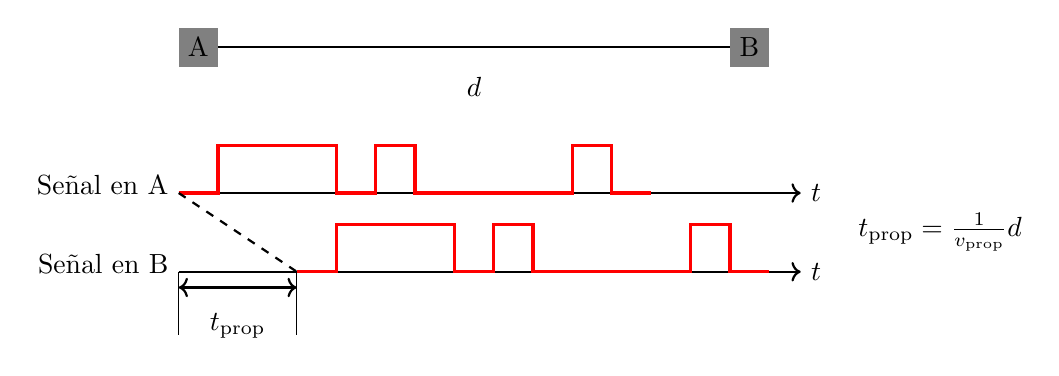
\begin{tikzpicture}[thick]
    % Top diagram: A and B with distance d
    \fill[gray] (0,3) rectangle (0.5,3.5);
    \node at (0.25,3.25) {A};
    \fill[gray] (7,3) rectangle (7.5,3.5);
    \node at (7.25,3.25) {B};
    \draw (0.5,3.25) -- (7,3.25);
    \node[below] at (3.75,3) {$d$};

    % Signal at A (y=1 low, y=2 high)
    \draw[->] (0,1.4) -- (7.9,1.4);
    \draw[line width=1.2pt, color=red] (0,1.4) -- (0.5,1.4) -- (0.5,2) -- (2,2) -- (2,1.4) -- (2.5,1.4) -- (2.5,2) -- (3,2) -- (3,1.4) -- (5,1.4) -- (5,2) -- (5.5,2) -- (5.5,1.4) -- (6,1.4);

    % Signal at B (y=0 low, y=1 high), shifted by 1 unit
    \draw[->] (0,0.4) -- (7.9,0.4);
    \draw[line width=1.2pt, color=red] (1.5,0.4) -- (2,0.4) -- (2,1) -- (3.5,1) -- (3.5,0.4) -- (4,0.4) -- (4,1) -- (4.5,1) -- (4.5,0.4) -- (6.5,0.4) -- (6.5,1) -- (7,1) -- (7,0.4) -- (7.5,0.4);

    % Dashed line connecting starts
    \draw[dashed] (0,1.4) -- (1.5,0.4);

    % t_prop label with arrows under the dashed line
    \draw[<->] (0,0.2) -- (1.5,0.2);
    \node[below] at (0.75,0) {$t_{\mathrm{prop}}$};
    \draw[thin] (0,0.4) -- (0,-0.4);
    \draw[thin] (1.5,0.4) -- (1.5,-0.4);

    % Labels
    \node[left] at (0,1.5) {Se\~{n}al en A};
    \node[left] at (0,0.5) {Se\~{n}al en B};

    % Time axis label
    \node[right] at (7.9,1.4) {$t$};
    \node[right] at (7.9,0.4) {$t$};
    \node[right] at (8.5,0.9) {$t_{\mathrm{prop}} = \frac{1}{v_{\mathrm{prop}}}d$};
\end{tikzpicture}


\begin{multicols}{2}
    \begin{tcolorbox}[title=Características fuente]
        \begin{tabular}{rl}
            \textbf{Alfabeto}:     & $X = \left\{ x_1, x_2, \ldots x_S \right\}$ \\
            \textbf{Probabilidad}: & $p_i : 0 \leq p_i \leq 1, \sum_{i=1}^{S}{p_i} = 1$ \\
            \textbf{Información}:  & $I_i = \log_2{\frac{1}{p_i}} = -\log_2{p_i}$ \\
                        & $I_i \geq 0$ para cualquier $0 \leq p_i \leq 1$ \\
                        & $I_i \to 0$ cuando $p_i \to 1$ \\
            \textbf{Entropía}:     & $H(X) = \sum_{i=1}^{S}{p_i \cdot I_i} = \sum_{i=1}^{S}{p_i \cdot \log_2{\frac{1}{p_i}}}$ \\
                        & $0 \leq H(X) \leq \log_2{S}$ \\
        \textbf{Longitud media}: & $\overline{L} = \sum_{i=1}^{S}{p_i \cdot L_i}$ \\
                        & en codificación longitud fija $\overline{L} = \lceil\log_2{S}\rceil$ \\
            \textbf{Eficiencia}:   & $\eta = \frac{H(X)}{\overline{L}}$
        \end{tabular}
    \end{tcolorbox}
    \begin{tcolorbox}[title=Entropía binaria]
        $S = 2$ \\
        $\eta = \frac{H(X)}{\overline{L}} = \Omega\left(p\right)$ \\
        $H(X) = \Omega\left(p\right) = p\cdot\log_2{\frac{1}{p}} + (1-p)\cdot\log_2\frac{1}{1-p}$ \\
        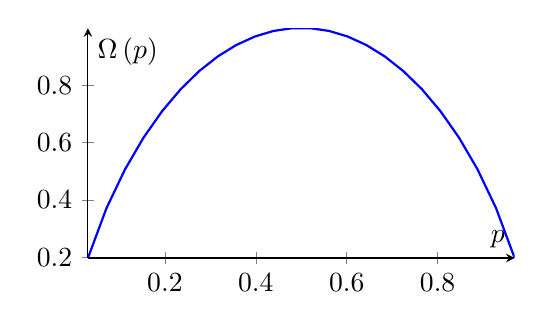
\begin{tikzpicture}
            \begin{axis}[
                width=7cm, height=4.5cm,
                axis lines = middle,
                xlabel=$p$, ylabel=$\Omega\left(p\right)$,
                domain=-0.5:1.5, samples=50,
                grid=none
            ]
            \addplot[blue, thick] {x*log2(1/x) + (1-x)*log2(1/(1-x))};
            \end{axis}
        \end{tikzpicture}
    \end{tcolorbox}
\end{multicols}

\begin{tcolorbox}[title=Enfoque probabilístico]
    \begin{tabularx}{\linewidth}{X X}
        \begin{tabular}{rl}
            \multicolumn{2}{l}{\bfseries Probabilidades absolutas} \\
            $p(x_i)$: & probabilidad fuente envíe símbolo $x_i$ \\
            $p(y_j)$: & probabilidad destinatario reciba el símbolo $y_j$
        \end{tabular}
        &
        \begin{tabular}{rl}
            \multicolumn{2}{l}{\bfseries Probabilidades condicionadas} \\
            $p(y_j \vert x_i)$: & probabilidad transición hacia delante \\
            $p(x_i \vert y_j)$: & probabilidad transición hacia atrás
        \end{tabular}
        \\\vspace{1pt}
        \begin{tabular}{rl}
            \multicolumn{2}{l}{\bfseries Aplicación teoremas básicos} \\
            Bayes: & $p(x_i,y_j) = p(y_j \vert x_i) \cdot p(x_i) = p(x_i \vert y_j) \cdot p(y_j)$ \\
            Prob.\ total: & $p(y_j) = \sum_{i=1}^{S}{p(y_j \vert x_i) \cdot p(x_i)}$ \\
                          & $p(x_i) = \sum_{i=1}^{N}{p(x_i \vert y_j) \cdot p(y_j)}$
        \end{tabular}
    \end{tabularx}
\end{tcolorbox}

\begin{tcolorbox}[title=Canal discreto]
    \textbf{Información mútua} \\
    Cantidad de información que ha transmitido el canal cuando la fuente envía el símbolo $x_i$ y la fuente recibe el símbolo $y_j$.
    \[
        I(x_i;y_j) = \log_2{\frac{1}{p(x_i)}} - \log_2{\frac{1}{p(x_i \vert y_j)}} = \log_2{\frac{p(x_i \vert y_j)}{p(x_i)}} = \log_2{\frac{p(y_j \vert x_i)}{p(y_j)}}
    \]

    \textbf{Información mútua media} \\
    \[
        I(X;Y) = \sum_{i=1}^{S}\sum_{j=1}^{N}{p(x_i,y_j) \cdot I(x_i;y_j)}
    \]

    \textbf{Equivocación} \\
    \[
        H(X \vert Y) = \sum\limits_{i=1}^{S}\sum\limits_{j=1}^{N}{p(x_i,y_j)\log_2{\frac{1}{p(x_i \vert y_j)}}}
    \]

    Al promediar tenemos:
    \[
        \left.
        \begin{array}{rl}
            I(x_i;y_j) \to & I(X;Y) \\
            \log_2{\frac{1}{p(x_i)}} \to & H(X) \\
            \log_2{\frac{1}{p(x_i \vert y_j)}} \to & H(X \vert Y)
        \end{array}
        \right\}
        I(X;Y) = H(X) - H(X \vert Y)
    \]

    \textbf{Capacidad} \\
    Máxima cantidad de bits de información por símbolo
    \[
        C = \max\limits_{p(x_i), p(y_j \vert x_i)}{I(X;Y)}
    \]
\end{tcolorbox}

\end{document}